\documentclass[12pt]{article}

\usepackage[margin=1in]{geometry}
\usepackage{authblk}
\usepackage{booktabs}
\usepackage{graphicx}
\usepackage{setspace}
\usepackage{textcomp}
\usepackage{xurl}
\usepackage{ragged2e}
\usepackage[justification=RaggedRight,singlelinecheck=false]{caption}
\usepackage[numbers,sort&compress]{natbib}

\doublespacing
\raggedbottom
\setlength{\RaggedRightParindent}{\parindent}
\setlength{\RaggedRightRightskip}{0pt plus 4em}
\setlength{\emergencystretch}{3em}
\clubpenalty=10000
\widowpenalty=10000
\displaywidowpenalty=10000

\newcommand{\keywords}[1]{\par\noindent\textbf{Keywords:} #1\par}
\newcommand{\sectionstatement}[2]{%
  \section*{#1}
  #2
}

\begin{document}

\title{Interpretable machine learning identifies amino acid states and substitutions associated with H3N2 antigenic variation}

\author[1,2]{Austin G. Meyer}
\author[3]{Mauricio Santillana}

\affil[1]{Department of Pediatrics, Baylor Scott \& White Medical Center, McLane Children's Hospital, Temple, TX, USA}
\affil[2]{Department of Pediatrics, Baylor College of Medicine, Temple, TX, USA}
\affil[3]{Department of Physics, Northeastern University, Boston, MA, USA}

\date{}

\maketitle
\RaggedRight

\sectionstatement{Correspondence}{Correspondence should be addressed to Austin G. Meyer.\par\noindent E-mail: austin.g.meyer@gmail.com}

\clearpage
\begin{abstract}
\RaggedRight
Seasonal influenza A(H3N2) vaccine updates are guided primarily by antigenic measurements such as hemagglutination inhibition titers. Sequence data can help identify emerging hemagglutinin substitutions for serological follow-up, but published analyses disagree on which positions carry the strongest antigenic signal. Here, we trained gradient-boosted tree models to predict standardized titer reductions from paired virus and antiserum hemagglutinin sequences in the Neher/Bedford benchmark and a larger WHO Collaborating Centre dataset. We used feature-attribution scores to quantify the contributions of site mismatches, amino-acid states, and directed substitutions. The Neher/Bedford models recovered the canonical cluster-transition positions. Passage-filtered Collaborating Centre models ranked a related, more contemporary set of head-region positions, including site 225, which a published structurally aware analysis had identified at high posterior inclusion probability. The rankings overlapped published antigenic site lists and several rankings derived without HI measurements. We evaluated the models by retrospective cross-validation and kept all observations of each named virus in the same fold. The training and test data could include the same sera and closely related viruses. We did not test performance on new clades or future seasons. The attributions describe associations with predicted titers. Together with substitution-level tables and exploratory predictions of background-dependent titer changes, they provide a framework for identifying sequence changes for further serological study.
\end{abstract}

\keywords{influenza A(H3N2) $|$ antigenic drift $|$ hemagglutination inhibition $|$ machine learning $|$ SHAP $|$ hemagglutinin}

\clearpage
\section{Introduction}

Seasonal influenza A(H3N2) vaccine strain selection is driven primarily by antigenic phenotype. Viruses are tested in hemagglutination inhibition (HI) assays against antisera raised against vaccine and reference strains, and these measurements guide vaccine updates~\cite{Russell2008Science, Bedford2015Nature, Smith2004Science}. Sequence data help identify viruses for serological follow-up. A newly sequenced virus carrying a substitution at a position with established antigenic significance provides a clear reason for further testing. The significance of substitutions at other positions is harder to assess. A more complete understanding of which hemagglutinin (HA) positions, and which substitutions at those positions, are associated with HI titer change would improve this decision process.

Published sets of important sites disagree more than one might expect. Early crystallographic and antibody-mapping studies defined four antigenic regions on H3 hemagglutinin (sites A--D)~\cite{Wiley1981Nature}; the canonical map is often described as five regions (sites A--E)~\cite{Koel2013Science}. Positive-selection analyses informed predictions of H3N2 evolution~\cite{bush1999predicting}, while cluster-transition analyses narrowed attention to a small number of receptor-binding-proximal positions~\cite{Koel2013Science}. Additive titer models built within phylogenetic frameworks implicated a broader set of positions~\cite{Neher2016PNAS}. A Bayesian structural-genomic analysis of WHO Collaborating Centre (WIC) HI data prioritized positions using posterior inclusion probabilities~\cite{Harvey2023PLoSComputBiol}, and a seasonal AdaBoost model trained on partially overlapping WIC data identified 30 positions through feature importance aggregated across influenza seasons~\cite{shah2024seasonal}. These four reference sets (Koel, Neher/Bedford, Harvey, and Shah) overlap at their core but diverge elsewhere. That divergence likely reflects differences in dataset composition, time period, analytical method, and passage-associated differences in HI reactivity~\cite{Parker2016JGenVirol} and antibody recognition~\cite{Zost2017PNAS}.

A separate class of approaches uses evolutionary variability as a proxy for antigenic importance. Sitewise dN/dS, the ratio of amino acid-changing to silent substitution rates, and Shannon entropy identify rapidly evolving or unusually variable positions~\cite{fitch1991positive, NeiGojobori1986, suzuki2006natural, pan2011quantifying}. Their relationship to antigenic effect is indirect. Interpretation is complicated by passage artifacts~\cite{McWhite2016VE_passage}, structural constraints that limit site variability independently of antigenic pressure~\cite{Meyer2015PP_geom, echave2016causes}, and rate estimation artifacts at short divergence times~\cite{Meyer2015VE_time, Ho2005MBE}. Statistical and machine learning approaches offer a more direct route. Sequence-based models have been applied to predict antigenic phenotype~\cite{xia2021deep} and influenza fitness~\cite{Luksza2014Nature}, and to inform vaccine-strain prediction~\cite{Steinbruck2014JVirol}. Interpretable methods have also been used to prioritize residues from protein-sequence data~\cite{hie2021learning, thadani2023learning}. Here, we ask whether applying a common modeling framework and consistent importance definitions to more than one HI collection can help explain agreement and disagreement among existing H3N2 site lists.

Most published rankings stop at the position level, although different amino acid substitutions at the same position can have different antigenic effects. Koel et al.\ showed experimentally that substitutions at position 145 were context-independent in their reverse-genetics panel, whereas substitutions at position 155 were context-dependent~\cite{Koel2019JGenVirol}. Substitution-level analyses can represent these differences and distinguish changes that add or remove glycosylation potential. For surveillance, the relevant question may concern a specific change such as N145K in a given season, beyond the general importance of site 145.

Here we apply gradient-boosted tree models (LightGBM) with SHAP-based attribution~\cite{Lundberg2017, Lundberg2020NatMachIntell} to the Neher/Bedford H3N2 dataset~\cite{Neher2016PNAS} and the larger WIC H3N2 dataset~\cite{Harvey2023PLoSComputBiol}. At each HA position, the models encode whether the virus and serum amino acids differ and which amino acid each carries. A separate encoding represents each directed substitution. SHAP values quantify the contribution of each feature to the predicted titer. We compare the resulting rankings with the Koel, Neher/Bedford, Harvey, and Shah reference sets, independent rankings derived without HI measurements~\cite{Meyer2026Interface_sequenceML}, and standard evolutionary metrics. For Harvey, we use all 14 HA1 positions with posterior inclusion probability (PIP) at least 0.95 in the structurally aware model, including 225~\cite{Harvey2023PLoSComputBiol}. In the supplement, we report exploratory computational introductions of Koel substitutions and site-160 glycosylation-motif changes. These analyses describe predicted titer changes across sequence backgrounds; experimental epistasis remains untested.

\section{Results}

\subsection{Interpretable models recover the canonical H3N2 cluster-transition sites from the Neher/Bedford dataset}

We first examined whether a common modeling framework could recover the canonical H3N2 cluster-transition sites from the Neher/Bedford data. We used two complementary LightGBM encodings. The site-state model represents each HA position with a binary change indicator and separate one-hot encodings of the virus and serum amino acids. The substitution model represents each observed directed amino-acid difference as a binary feature, such as a covariate for N145K. Both include temporal distance. We evaluated the models by five-fold cross-validation grouped by virus name, assigning all observations for a given virus to the same fold. We used this procedure to evaluate retrospective predictions for held-out named viruses. We describe the scope of this evaluation in Methods.

The Neher/Bedford H3N2 dataset contains 8{,}599 HI measurements after exact strain-name matching to HA sequences, alignment, and quality control, with viruses and antisera spanning 1968 through 2011. We trained the models to predict residual standardized log\textsubscript{2} HI titers after removing per-serum and per-virus additive offsets (Table~\ref{tab:primary-model-summary}). The site-state model achieved a mean cross-validation Spearman correlation of 0.714 and RMSE of 1.971 log\textsubscript{2} titer units. The substitution model performed comparably, with a Spearman correlation of 0.704 and RMSE of 2.046. Both exceeded the temporal-distance-only baseline (Spearman 0.587), indicating that HA sequence variation carries predictive information beyond calendar time.

\begin{table}[t]
\centering
\caption{Predictive performance of the primary models. HI observations are virus--serum pairs retained after matching both components to HA sequences and applying alignment quality control (see Methods). Values are mean RMSE and Spearman correlation between predicted and observed standardized log\textsubscript{2} HI titers across held-out folds of cross-validation grouped by virus name.}
\label{tab:primary-model-summary}
\small
\begin{tabular}{lrrrr}
\toprule
Dataset & HI observations & Model & RMSE & Spearman \\
\midrule
Neher/Bedford H3N2 & 8{,}599 & site-state & 1.971 & 0.714 \\
 &  & substitution & 2.046 & 0.704 \\
WIC H3N2 & 104{,}605 & site-state + context & 1.234 & 0.809 \\
 &  & substitution + context & 1.263 & 0.799 \\
WIC H3N2 (filtered) & 28{,}448 & site-state + context & 0.992 & 0.782 \\
 &  & substitution + context & 1.002 & 0.779 \\
\bottomrule
\end{tabular}
\par\vspace{0.4em}
\begin{minipage}{\textwidth}
\raggedright\footnotesize
\textit{Note:} The filtered WIC analysis excludes observations whose normalized virus or reference passage class is exactly \texttt{EGG}, \texttt{MIXED}, or \texttt{UNKNOWN}. Filtering changes the response distribution, which prevents direct comparison of RMSE and Spearman values between the unfiltered and filtered rows (see Methods). ``Context'' indicates assay-context covariates included alongside sequence features after an additive avidity/potency correction (see Methods). Neher/Bedford positions use mature HA numbering, excluding the 16-residue signal peptide. Table~S1 provides full results, including patristic-distance sensitivity analyses.
\end{minipage}
\normalsize
\end{table}

We used SHAP values to quantify the contribution of each feature to the predicted titer for a given virus--serum pair~\cite{Lundberg2017, Lundberg2020NatMachIntell}. Large mean absolute SHAP values identify sites whose sequence states most consistently predict antigenic distance in the fitted model. Correlated HA substitutions along clades can share this predictive signal, so the attribution to a site does not establish its independent causal effect.

The leading sites in the site-state model were head-region positions associated with H3N2 cluster transitions (Fig.~\ref{fig:h3n2-primary}), including 189, 145, 133, 135, 121, 158, 156, 193, and 144. Of the seven Koel cluster-transition positions (145, 155, 156, 158, 159, 189, 193)~\cite{Koel2013Science}, six appeared among the site-state model's top 30 and all seven appeared in the substitution model's top 30 (Table~S2). We found 11 of the 15 Neher/Bedford reference positions compiled from substitutions discussed by Neher et al.~\cite{Neher2016PNAS} in the site-state top 30 and 14 in the substitution top 30. Both encodings recovered 12 of the 14 Harvey structurally aware PIP~$\geq$0.95 positions~\cite{Harvey2023PLoSComputBiol}; the site-state model also recovered 14 of 30 Shah positions (Table~S2). For comparison, two independently drawn sets of 30 from 550 mature-HA sites would overlap by 1.6 sites on average (0.4 for a 7-site list; 0.8 for a 15-site list). The leading positions had stable ranks across folds (Fig.~S3). In a secondary grouped-virus holdout that withheld 10\% of virus names at once, the sequence models again outperformed the non-sequence baseline (Fig.~S1). This holdout has the same relatedness limitation as the primary cross-validation. Fig.~S4 compares predicted and observed titers for the random-measurement and grouped-virus holdouts.

\begin{figure}[t]
\RaggedRight
\noindent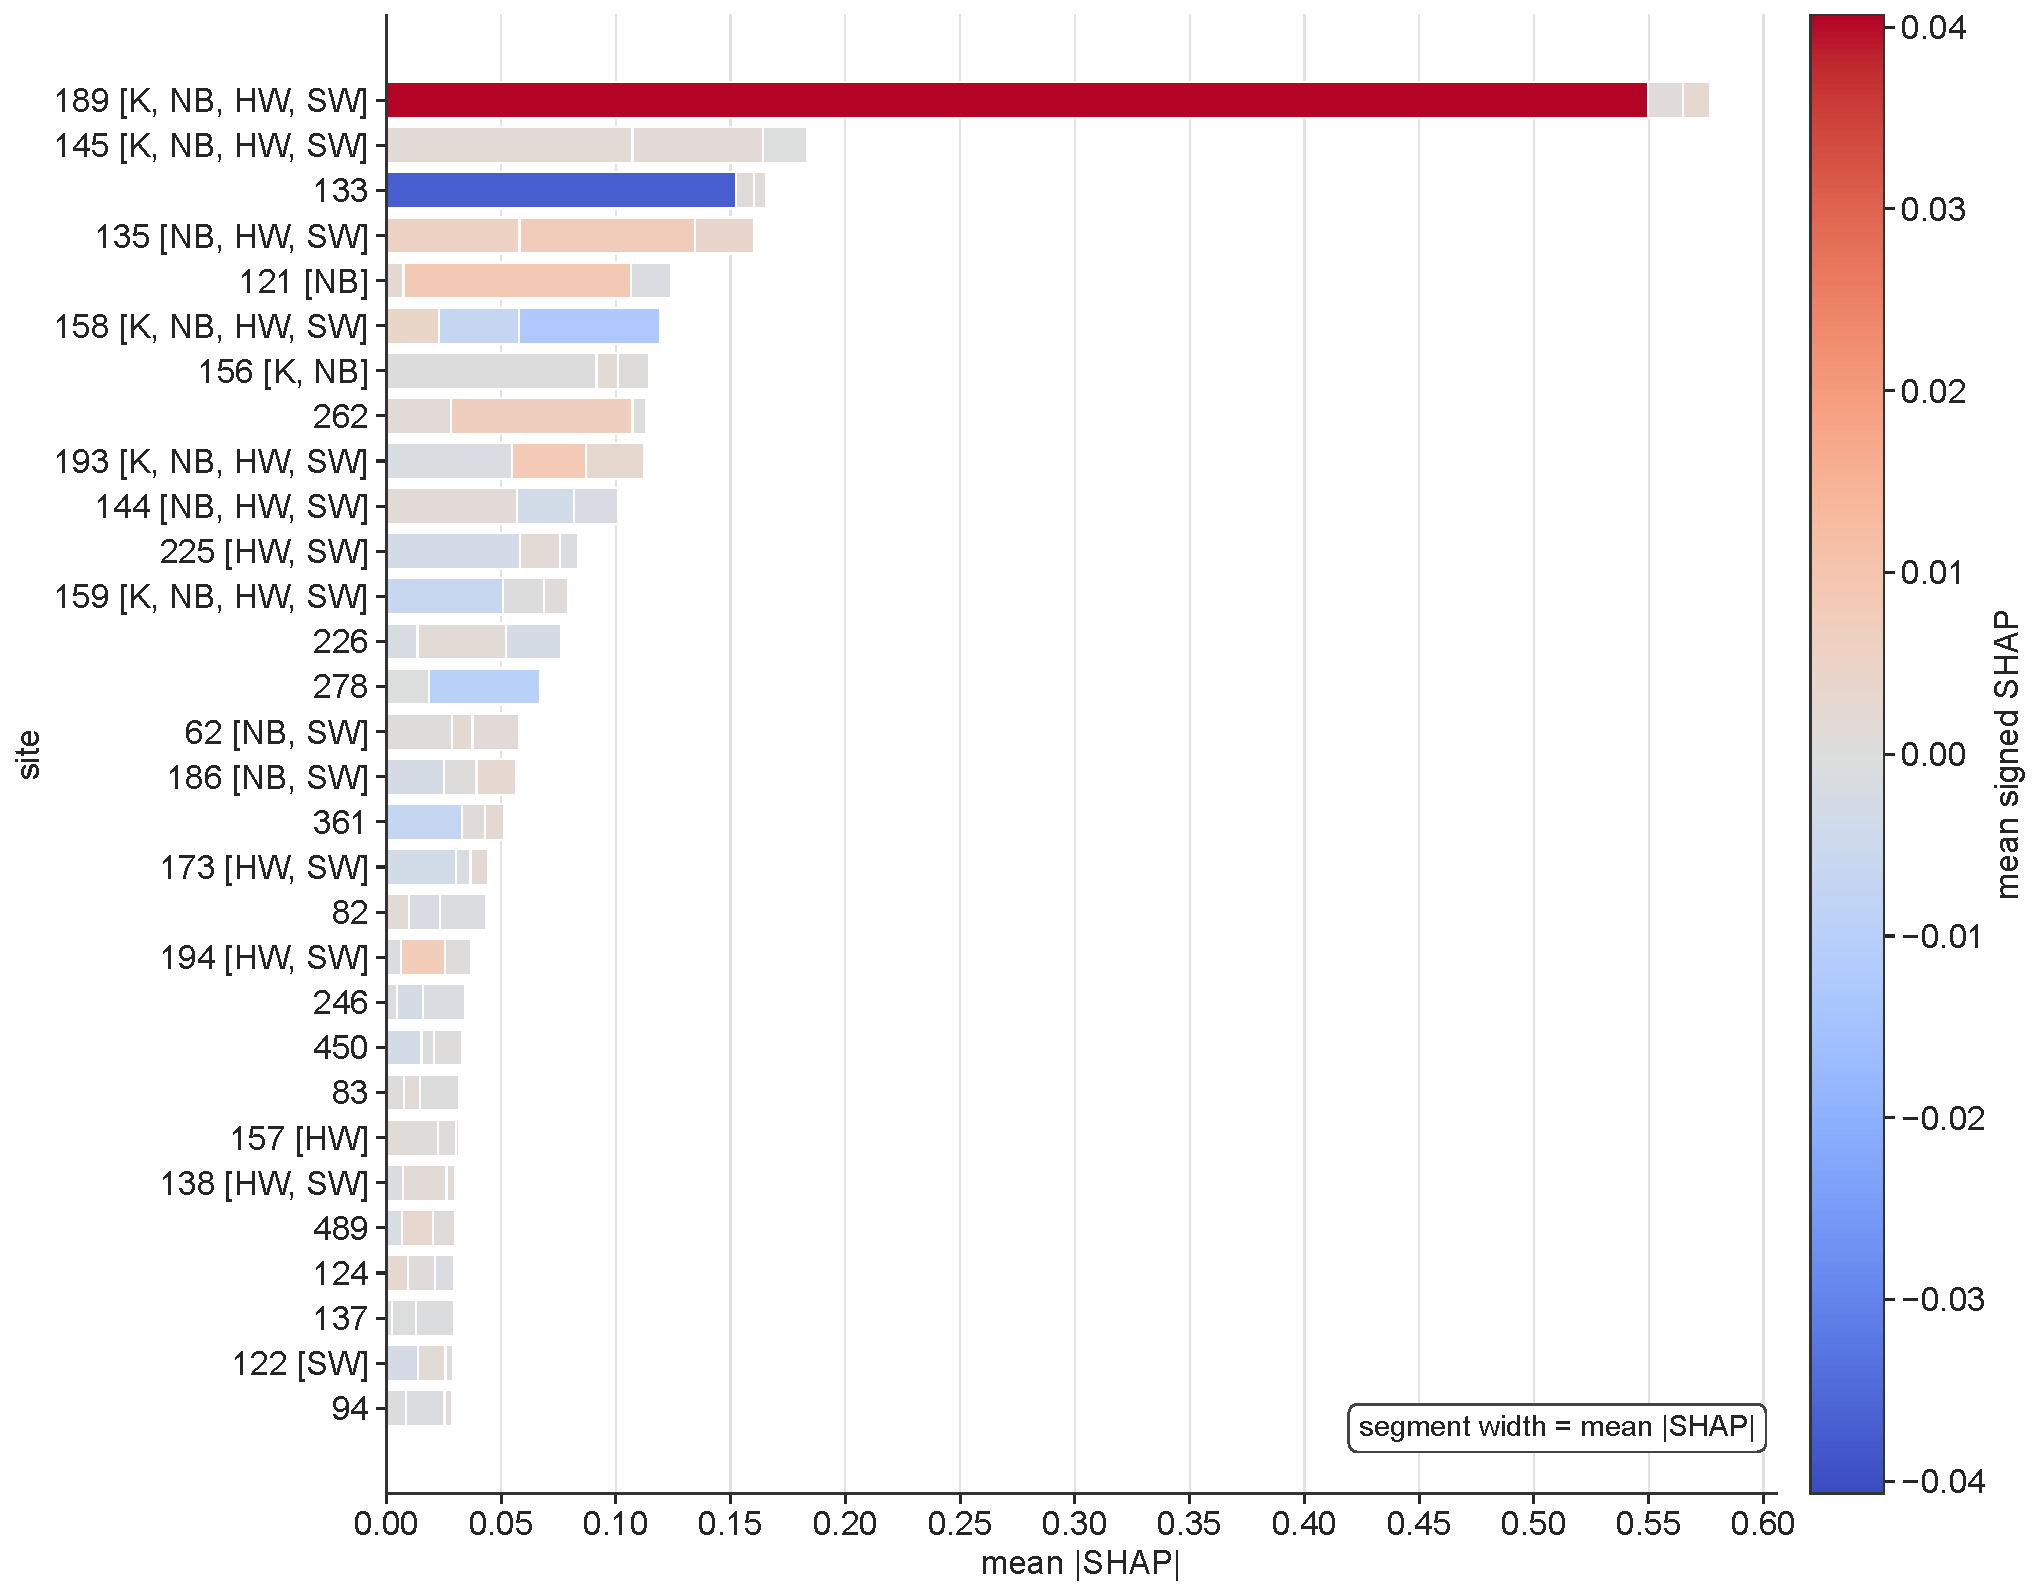
\includegraphics[width=\textwidth]{figures/fig1_h3n2_site_component_top30.pdf}
\caption{Site-level SHAP decomposition for the Neher/Bedford site-state model. Bars show the top 30 mature-HA sites ranked by mean absolute SHAP value across grouped-cross-validation folds. Segments show the contributions of site-change, virus-state, and serum-state features to each site's total score. Segment color represents mean signed SHAP, using the scale at right. Brackets beside each site label show membership in the Koel reference set (K; 7 positions), the Neher/Bedford reference set (NB; 15 positions), the Harvey structurally aware PIP~$\geq$0.95 set (HW; 14 positions), and the Shah reference set (SW; 30 positions). Leading positions include the canonical cluster-transition sites 189, 145, 156, 158, 159, and 193. All positions use mature HA numbering, excluding the N-terminal 16-residue signal peptide.}
\label{fig:h3n2-primary}
\par\vspace{0.35em}
\noindent\textit{Alt text.} Horizontal stacked bars rank the top 30 hemagglutinin sites from the Neher/Bedford site-state model by mean absolute SHAP value, with segments for change, virus-state, and serum-state contributions and literature-set brackets beside the site labels. Segment color represents mean signed SHAP.
\end{figure}

Adding patristic distance as a covariate had little effect on performance (Spearman 0.715 and RMSE 1.973 with patristic distance, compared with 0.714 and 1.971 without; Table~S1) or on the leading sites (Fig.~S12, S13). Thus, the Neher/Bedford site-state model recovered the canonical cluster-transition site set from HI titers and HA sequences, using neither structural data nor an explicit phylogenetic correction.

\subsection{Passage filtering clarifies the biological signal in the WIC dataset}

We next applied the models to the larger WIC H3N2 dataset. These virus--serum HI observations span multiple decades, although most modeled observations were collected after 2010. Of the 202{,}605 raw HI observations, 104{,}972 (51.8\%) had matched HA1 sequences for both virus and serum components, and 104{,}605 (51.6\%) passed alignment quality control. Egg passage can alter measured HI reactivity~\cite{Parker2016JGenVirol} and antibody recognition~\cite{Zost2017PNAS}, complicating interpretation of the circulating virus.

We therefore filtered the WIC observations by passage history, excluding those whose normalized virus or reference passage class was exactly \texttt{EGG}, \texttt{MIXED}, or \texttt{UNKNOWN}. We retained 28{,}521 sequence-matched measurements after filtering, of which 28{,}448 passed alignment quality control (Table~S3). The rule retains composite labels such as \texttt{CELL|EGG}. A stricter rule excluding any label containing \texttt{EGG} would remove another 418 of 28{,}521 rows (1.5\%), leaving 28{,}103. We counted these additional exclusions but did not retrain under the stricter rule (Supplementary Methods S1.8). We therefore used the exact-class filter for the primary analysis. This smaller subset is enriched for recent, cell-associated observations and offers clearer interpretation at the cost of reduced representativeness.

In the passage-filtered WIC data, the site-state model achieved a mean cross-validation Spearman correlation of 0.782 and RMSE of 0.992 (Table~\ref{tab:primary-model-summary}; Table~S1). The unfiltered model had a higher Spearman correlation (0.809) and RMSE (1.234). Because filtering changes the response distribution, these metrics cannot be compared directly across subsets. The predicted-versus-actual scatter provides a clearer view of the change. Predictions for the filtered data form a tighter distribution, and the two-cluster structure seen in the unfiltered data is absent (Fig.~S6, S10). We use the filtered models as the primary contemporary analysis.

The leading sites in the filtered site-state model were 144, 225, 159, 140, and 145. Sites 142, 62, 53, 45, 326, 197, 158, 193, 173, and 189 also appeared among the top 15 (Fig.~\ref{fig:wic-filtered-primary}). Site 144 belongs to antigenic region A and the Harvey PIP~$\geq$0.95 set~\cite{Harvey2023PLoSComputBiol}. Site 225 ranked second; Harvey et al.\ included it among the 14 structurally aware PIP~$\geq$0.95 positions and classified it as part of the receptor-binding site. The leading sites had stable ranks across folds (Fig.~S7), and Fig.~S8 compares standardized with context-corrected titers. Sequence models also outperformed the context-only baseline in a secondary grouped-virus holdout (Fig.~S5). Fig.~S9 compares predicted and observed titers for the random-measurement and grouped-virus holdouts.

\begin{figure}[t]
\RaggedRight
\noindent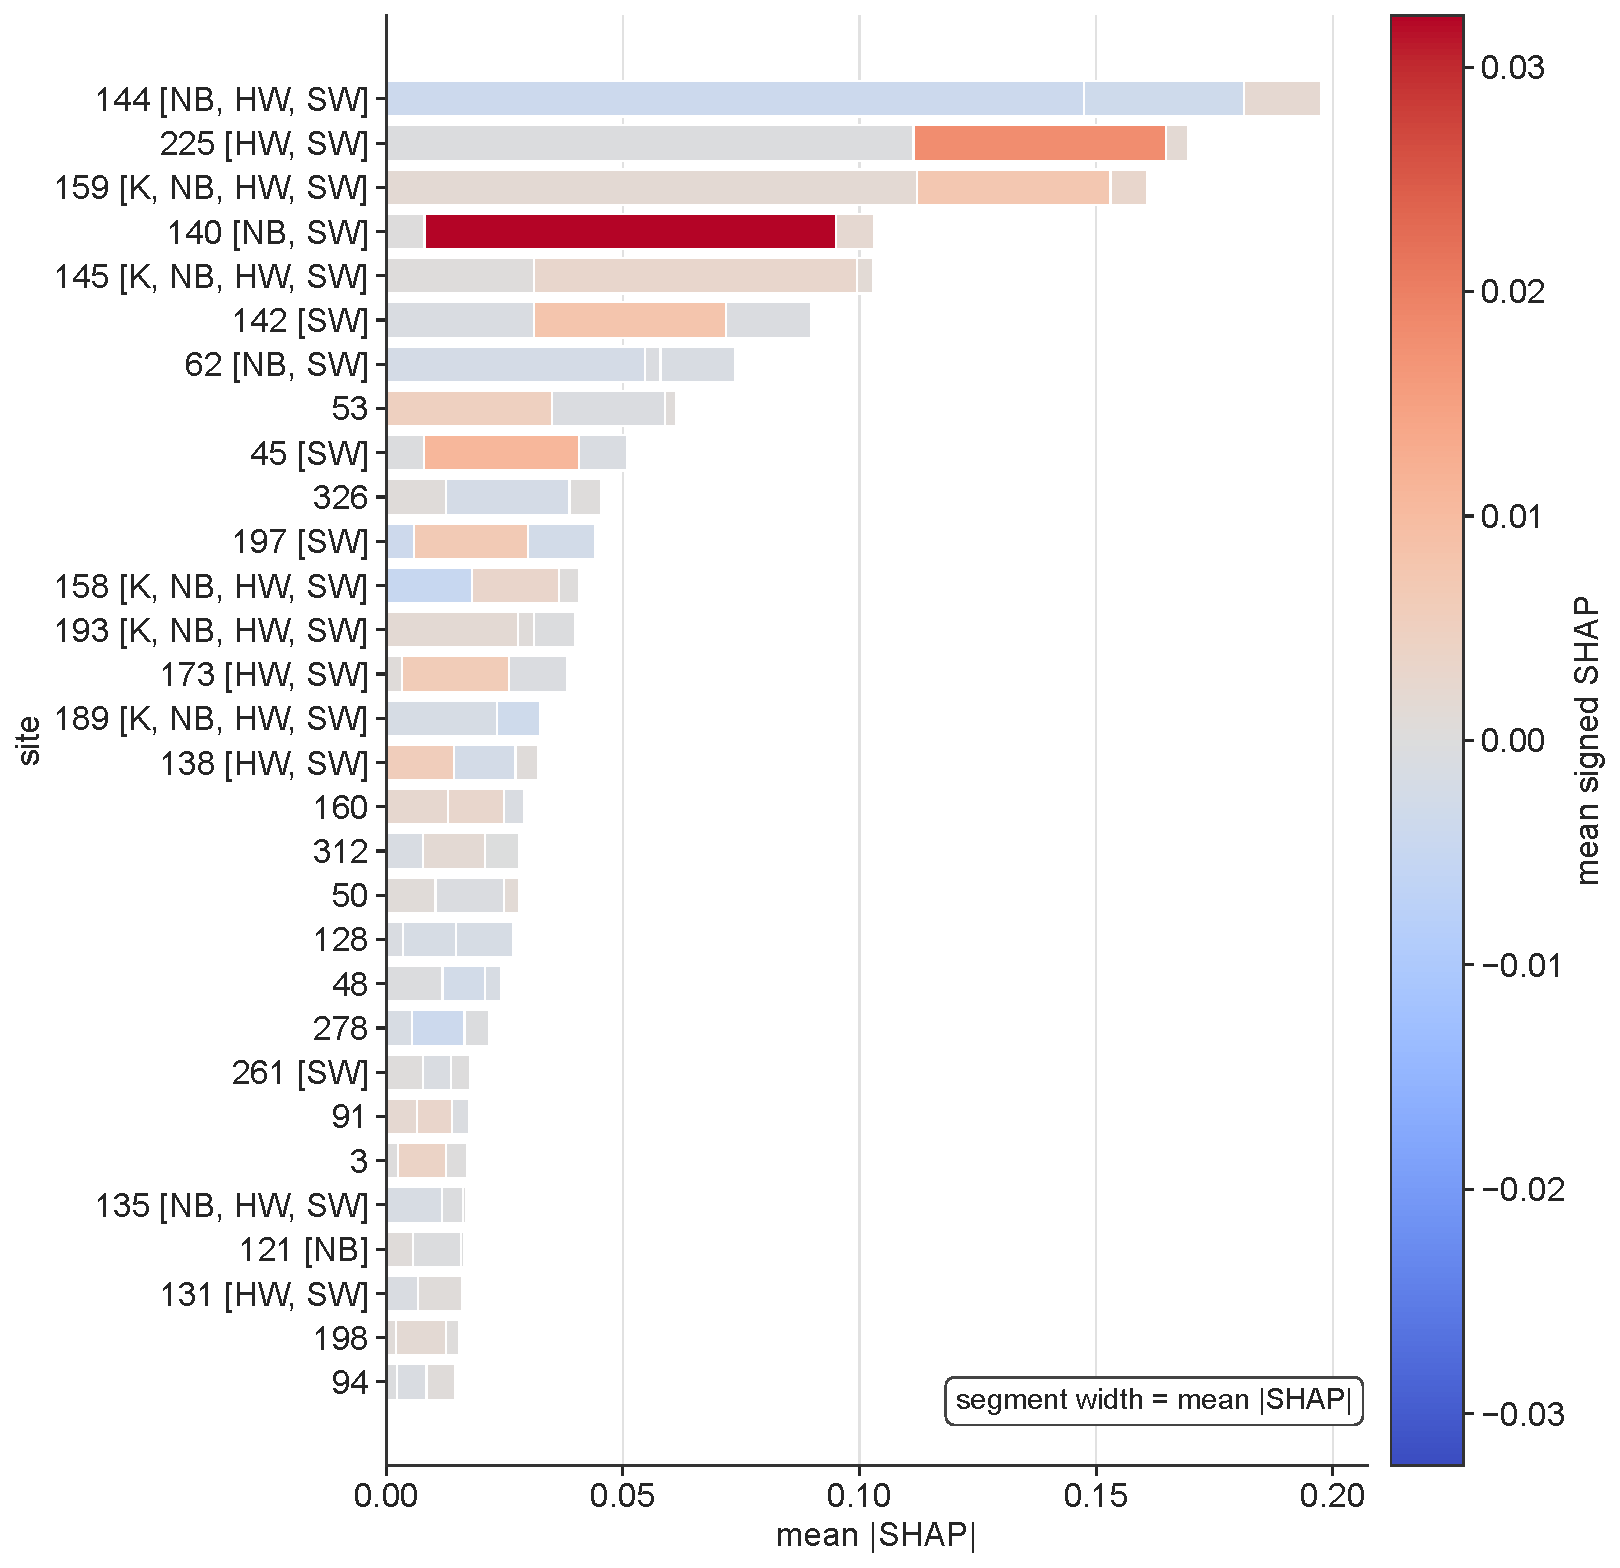
\includegraphics[width=\textwidth]{figures/fig2_wic_filtered_site_component_top30.pdf}
\caption{Site-level SHAP decomposition for the passage-filtered WIC site-state model. Bars show the top 30 HA1 sites ranked by mean absolute SHAP value across grouped-cross-validation folds. Segment width represents mean absolute SHAP, and color represents mean signed SHAP. Brackets beside the site labels show reference-set membership, as in Fig.~\ref{fig:h3n2-primary}; Harvey brackets use the 14-site PIP~$\geq$0.95 set. The filter excludes rows whose normalized virus or reference passage class is exactly \texttt{EGG}, \texttt{MIXED}, or \texttt{UNKNOWN}. Site 225 ranks second and is among Harvey et al.'s structurally aware PIP~$\geq$0.95 positions.}
\label{fig:wic-filtered-primary}
\par\vspace{0.35em}
\noindent\textit{Alt text.} Horizontal stacked bars rank the top 30 HA1 sites from the passage-filtered WIC site-state model by mean absolute SHAP value, with change, virus-state, and serum-state segments and literature-set brackets beside the site labels, led by sites 144, 225, and 159. Segment color represents mean signed SHAP.
\end{figure}

The unfiltered WIC rankings were noisier, with passage-associated positions more prominent alongside canonical antigenic sites (Fig.~S10, S11). Adding patristic distance to the filtered site-state model improved performance only slightly (Spearman 0.787 versus 0.782, RMSE 0.982 versus 0.992; Table~S1). Interpretability therefore depended more on which observations were retained than on phylogenetic correction.

\subsection{The models explain predictions at the level of specific amino-acid states and substitutions}

The feature-level SHAP values allow us to distinguish the contributions of amino-acid states and directed substitutions at each position. Figs.~\ref{fig:h3n2-primary} and \ref{fig:wic-filtered-primary} aggregate these components into site-level scores. Tables~S4 and S5 provide the complete value-level results.

In the Neher/Bedford analysis, a mismatch at site 189 was the most influential site-state feature, contributing a mean SHAP of 0.899 log\textsubscript{2} titer units toward greater antigenic distance across 2{,}823 observations. Among substitutions observed at that site, S189R had the largest positive contribution (mean SHAP 1.031; $n=254$). At site 158, N158K had the largest positive substitution-level contribution in that model (mean SHAP 1.561; $n=188$). The sign also carries information. K193S was associated with reduced predicted titer loss (mean SHAP $-1.188$; $n=92$). K383R, at a site in HA2, had the largest absolute substitution-level SHAP in the same table (mean SHAP $-1.655$; $n=46$). Its count of 46 refers to assay observations, which can include repeated observations of a virus. We retained sparse substitutions and their observation counts in the complete tables.

In the filtered WIC substitution model, K189N had the largest positive contribution (mean SHAP 1.724; $n=67$ in the 12{,}500-row SHAP subsample). Other signed examples included H197Q ($-0.833$; $n=187$) and N225D ($+0.831$; $n=1{,}099$). At site 145, N145S had the largest contribution ($+0.323$; $n=1{,}642$). Fig.~S16 and Fig.~S17 show the top 20 signed value-level features for both primary models. These values describe contributions to predictions from the fitted trees. We did not measure experimental effect sizes.

\subsection{Cross-study synthesis identifies a convergent set of antigenically informative H3N2 sites}

We compared the top 30 sites from each primary site-state model with the four benchmark sets and external rankings derived without HI measurements (Fig.~\ref{fig:cross-study-concordance}). The reference sets share a core of sites, with more limited pairwise overlap elsewhere. For Harvey and Shah, 13 of the 14 Harvey PIP~$\geq$0.95 sites appear in the Shah set, giving a union of 31. Table~S2 reports benchmark overlap counts. Table~S6 summarizes agreement with published lists for the union of each model's top 15 sites, providing a record of literature concordance.

\begin{figure}[t]
\RaggedRight
\noindent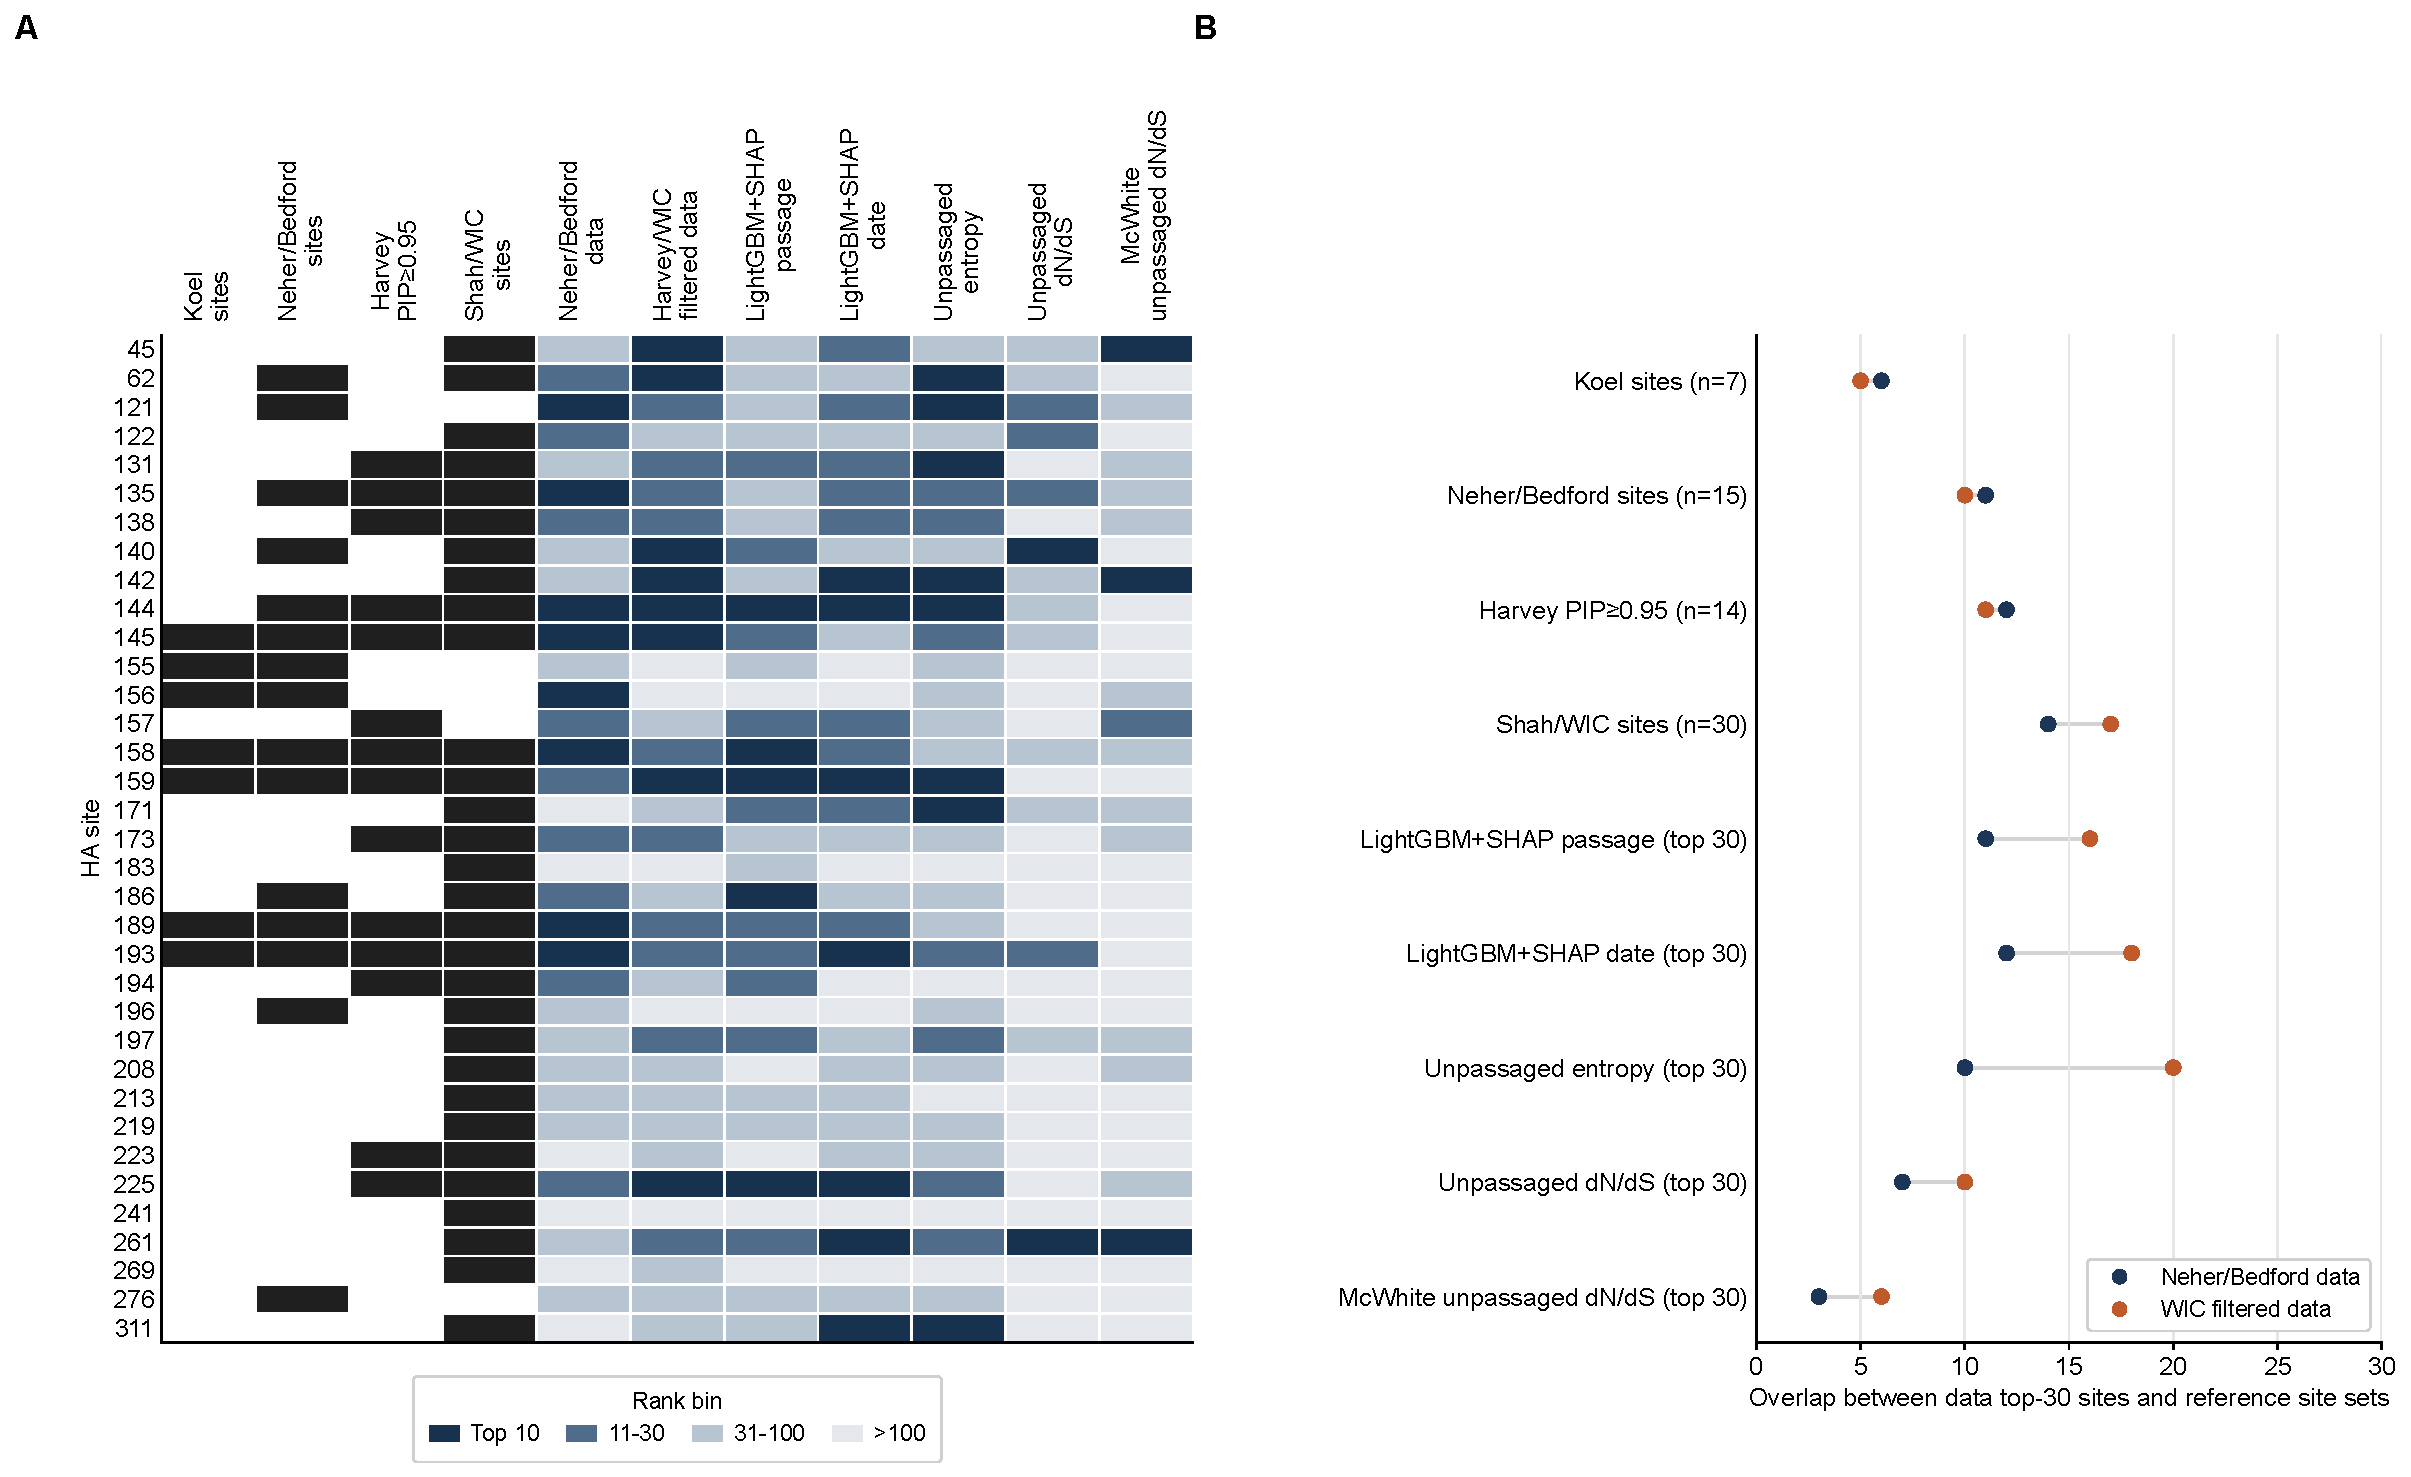
\includegraphics[width=\textwidth]{figures/fig3_cross_study_concordance.pdf}
\caption{Agreement between SHAP-based rankings and prior antigenic site sets. \textbf{(A)} Comparison across the union of Koel, Neher/Bedford, Harvey PIP~$\geq$0.95, and Shah reference positions. Each row is a site. The four reference-set columns mark membership in black. The remaining columns show rank tiers for the two site-state models and the external rankings, with darker shading for higher ranks. The bins are the top 10, 11--30, 31--100, and $>100$. \textbf{(B)} Overlap of each model's top-30 site set with each benchmark or external ranking. Horizontal position gives the number of matching sites out of the reference set size (7 for Koel; 15 for Neher/Bedford; 14 for Harvey PIP~$\geq$0.95; 30 for Shah and external rankings derived without HI measurements).}
\label{fig:cross-study-concordance}
\par\vspace{0.35em}
\noindent\textit{Alt text.} Panel A is a site-by-study heatmap of rank tiers and reference-set membership. Panel B plots how many of each reference set or external top-30 list derived without HI measurements overlap the Neher/Bedford and filtered WIC top-30 site-state rankings.
\end{figure}

The Neher/Bedford site-state model recovered 6 of 7 Koel positions, 11 of 15 Neher/\allowbreak Bedford positions, 12 of 14 Harvey PIP~$\geq$0.95 positions, and 14 of 30 Shah positions. The filtered WIC site-state model recovered 5 of 7 Koel positions, 10 of 15 Neher/Bedford positions, 11 of 14 Harvey positions, and 17 of 30 Shah positions (Table~S2). The machine-readable data accompanying Table~S2 also report a restricted 15-site Harvey variant that omits 225, labeled as a sensitivity comparison.

We also found substantial overlap between the filtered WIC top 30 and rankings derived without HI measurements. Models predicting passage history and collection date with LightGBM+SHAP~\cite{Meyer2026Interface_sequenceML} shared 16 and 18 of 30 positions, respectively, with the filtered WIC ranking. The most variable positions in unpassaged H3N2 sequences, measured by Shannon entropy, shared 20 of 30 (Fig.~\ref{fig:cross-study-concordance}B). Overlap was weaker for sitewise dN/dS, with 10 of 30 positions shared with the unpassaged dN/dS ranking and 6 of 30 with the McWhite et al.\ unpassaged ranking~\cite{McWhite2016VE_passage}.

The main conclusions were similar in two sensitivity analyses. Including all unfiltered WIC observations produced a noisier ranking (Fig.~S10, S11), while adding patristic distance had little effect on RMSE and retained substantial overlap among the leading sites (Table~S1; Fig.~S12--S15). Supplementary Results Section D reports exploratory predictions of background-dependent titer changes at Koel sites 145 and 155 and at the HA1 158--160 glycosylation motif.

\section{Discussion}

We found that gradient-boosted tree models with SHAP attribution recovered a large fraction of the positions identified in the Koel, Neher/Bedford, Harvey, and Shah H3N2 analyses. The models also described the contributions of amino-acid states and directed substitutions at those positions. The Neher/Bedford model recovered nearly all canonical cluster-transition sites~\cite{Koel2013Science, Neher2016PNAS}. The filtered WIC model shared 11 of Harvey's 14 structurally aware PIP~$\geq$0.95 sites, including 225, and 17 of Shah's 30 sites~\cite{Harvey2023PLoSComputBiol, shah2024seasonal}. Harvey and Shah already share 13 of those 14 Harvey sites. We applied the same framework to two HI collections and reported site, state, and substitution attributions under a common definition of each reference set.

For each site, we quantify the contributions of the amino-acid mismatch between the test virus and the serum-raised virus, the amino acid each virus carries, and each directed substitution. SHAP assigns a signed contribution to each component~\cite{Lundberg2017, Lundberg2020NatMachIntell}. Additive titer models, including the Neher/Bedford framework, represent genetic contributions to antigenic change as a sum of independent branch or substitution effects~\cite{Neher2016PNAS}. This works well when effects are approximately additive. Bayesian structural-genomic models such as Harvey et al.\ incorporate phylogenetic and structural information and account for uncertainty more formally~\cite{Harvey2023PLoSComputBiol}. Tree models can represent interactions through their splits. SHAP then decomposes the resulting prediction into feature contributions, whose interpretation remains tied to that fitted predictor.

Site 225 illustrates how to interpret these attributions alongside earlier work. It ranked second in the filtered WIC site-state model and first in the corresponding substitution model, where N225D had a mean SHAP of 0.831 across 1{,}099 observations in the SHAP subsample. Harvey et al.\ included 225 among the 14 structurally aware PIP~$\geq$0.95 positions and assigned it to the receptor-binding site~\cite{Harvey2023PLoSComputBiol}. Chambers et al.\ listed N225D among HA differences separating 2014--2015 3C.2a and 3C.3a viruses from A/Texas/50/2012. Their reverse-genetics panel identified antigenic-site-B mutations as the principal drivers of that mismatch~\cite{Chambers2015CellReports}. Thus, the high SHAP rank agrees with Harvey's PIP ranking and with the presence of N225D in those drift backgrounds. These comparisons provide observational and predictive support; they do not independently establish 225 as a classical epitope.

Agreement with rankings derived without HI measurements~\cite{Meyer2026Interface_sequenceML} is consistent with the prioritized sites being evolutionarily active. Shared confounding and correlated substitution patterns can also produce high ranks across analyses. The weaker overlap with dN/dS is expected if dN/dS identifies diversifying selection without distinguishing antigenic consequence~\cite{fitch1991positive, suzuki2006natural, echave2016causes, Meyer2015PP_geom, Meyer2013MBE}. Here, SHAP importance is tied to a measured HI outcome and therefore more closely matches the surveillance task of ranking substitutions by predicted titer association.

Two modeling choices also emerged. First, exact-class passage filtering produced a clearer contemporary ranking than the unfiltered WIC data, consistent with work showing that egg adaptation confounds residue-level analyses~\cite{Bush2000PNAS_passage, McWhite2016VE_passage, Parker2016JGenVirol, Zost2017PNAS, kistler2025MBE}. Composite egg labels account for 1.5\% of the rows retained by the primary filter. We did not retrain the models with these rows excluded. Second, patristic distance provided at most marginal improvement. A flexible nonlinear model can largely account for phylogenetic structure already present in the sequence features.

Both collections reflect surveillance sampling and assay preferences. The filtered WIC analysis retains 28{,}448 of 104{,}605 sequence-matched observations that pass alignment quality control. We used grouped cross-validation to evaluate retrospective predictions for held-out virus names. We did not test performance in future seasons. Highly ranked sites can reflect correlated clade structure, sampling, or assay context. Agreement with the four reference sets should therefore be interpreted as concordance across analyses. The Koel 2013 cluster-transition sites have an experimental basis, while the Koel 2019 experiments at 145/155 provide context for the exploratory predictions in the supplement. We did not reproduce those experiments as a signed-effect test. The encoding also leaves glycosylation occupancy unmodeled~\cite{Das2011PNAS_glycan, Kosik2018PLoSPathog, Altman2019mBio, Zost2017PNAS}. We retained sparse substitutions such as K383R and their observation counts in the complete tables. The supplement reports both full-data and cross-validation fits for the exploratory Koel counterfactuals; the main performance table reports cross-validation.

For surveillance, positions that rank highly across both datasets, both encodings, and multiple reference comparisons offer the strongest candidates for serological follow-up in newly circulating variants. Differences between datasets may reflect temporal or dataset-specific variation. Together with deep mutational scanning~\cite{Lee2018PNAS, Thyagarajan2014eLife} and antigenic cartography~\cite{Smith2004Science}, these rankings and value-level tables can help direct experiments toward substitutions most likely to be associated with HI titer change~\cite{Neher2016PNAS, Bedford2015Nature}.

\section{Materials and Methods}

\subsection{Data sources and sequence processing}

We obtained the Neher/Bedford H3N2 HI dataset and matched HA sequences from the Neher/Bedford antigenic and phylogenetic analysis framework~\cite{Neher2016PNAS}. We assembled the WIC H3N2 HI dataset and passage annotations from the WHO Collaborating Centre surveillance data described in Harvey et al.~\cite{Harvey2023PLoSComputBiol}.

For the Neher/Bedford dataset, we retrieved HA sequences from GISAID~\cite{Elbe2017GlobChall, Shu2017EuroSurveillance} using isolate identifiers matched to the HI records. We used NCBI GenBank as a fallback for isolates unresolved through GISAID. We normalized strain names to uppercase alphanumeric characters and matched sequences by exact normalized name, without fuzzy matching. After alignment quality control, the modeling dataset contained 8{,}599 HI observations and 402 HA sequence records corresponding to virus names. These records represented 338 distinct aligned amino-acid strings.

The 202{,}605 raw WIC HI observations reference 16{,}223 unique virus and reference serum strains, requiring a multi-stage sequence search. We first searched the curated HA1 alignment distributed with Harvey et al.~\cite{Harvey2023PLoSComputBiol}, which provided 1{,}738 matched sequences. We then searched GISAID manually by strain name~\cite{Elbe2017GlobChall, Shu2017EuroSurveillance}, obtaining 2{,}501 additional strain-level matches, and used NCBI GenBank/IRD and BV-BRC as fallback sources. The final modeling inputs contained 2{,}501 GISAID sequences and 1{,}738 Harvey repository sequences, representing 4{,}239 resolved strains. These yielded 104{,}972 HI observations with sequences for both components, of which 104{,}605 passed alignment quality control. When a strain name matched multiple GISAID isolates, we selected a canonical isolate by preferring HA1-complete sequences ($\geq 328$ residues), then lower-passage material (unpassaged $>$ cell $>$ egg), lower sequence ambiguity, and finally the most common variant among HA1-complete candidates.

For the Neher/Bedford dataset, we aligned HA protein sequences to A/\allowbreak HongKong/\allowbreak 1/\allowbreak 1968 using MAFFT~\cite{Katoh2013MolBiolEvol} in automatic mode, removed the N-terminal 16-residue signal peptide, and retained the 550-residue mature HA sequence. For WIC, we extracted HA1 sequences, aligned them with MAFFT, and mapped them to mature HA positions. We excluded sequences with more than 5\% gaps or more than 2\% ambiguous residues. Supplementary Methods S1.1 and S1.2 provide full details.

\subsection{Titer preprocessing and avidity/potency correction}

We first standardized each titer against the homologous titer of the corresponding serum, so that larger values indicate greater loss of cross-reactivity against heterologous viruses. Before log\textsubscript{2} transformation, we converted censored values reported as $<$X or $>$X to X/2 and 2X, respectively.

For Neher/Bedford, we applied an additive correction with serum identity and virus strain as categorical factors before interpreting sequence features. For WIC, we used passage history to define a filtered subset and to account for laboratory-specific and assay-specific titer offsets. We excluded observations when either the virus or reference serum had a normalized passage class exactly equal to \texttt{EGG}, \texttt{MIXED}, or \texttt{UNKNOWN}. We retained 28{,}521 sequence-matched observations, including 28{,}448 with aligned HA1 sequences. We then fitted an additive avidity/potency model jointly by ordinary least squares, using reference serum identity, assay-date label, virus passage class, reference serum passage class, antiserum class, and red blood cell type as six categorical factors. We re-estimated the additive layer within each training split. Supplementary Methods S1.3 provide full details.

\subsection{Feature encodings and model fitting}

We applied two complementary sequence encodings to each dataset, covering the 550-residue mature HA sequence for Neher/Bedford and the 328-residue HA1 alignment for WIC. The site-state encoding represents each position with a change indicator and separate one-hot encodings of the virus and serum amino-acid states. The substitution encoding represents each observed directed amino-acid change from serum to virus as a binary indicator. Neher/Bedford models included temporal distance, defined as the absolute calendar-year difference. WIC models included temporal distance and assay-context covariates. We added patristic distance in sensitivity analyses. Supplementary Methods S1.4 describe the encodings in full.

We trained gradient-boosted tree models using LightGBM~\cite{Ke2017LightGBM} with up to 1{,}000 boosting iterations, a learning rate of 0.1, 31 leaves, a minimum of 20 child samples, and no L1 or L2 regularization. Within each training split, we selected the number of boosting rounds using an inner group-based split that withheld 20\% of training virus names for early stopping. We evaluated performance by five-fold cross-validation grouped by virus name. All observations of a named virus remained in one fold, while sera could appear in several folds and closely related viruses could appear in both training and test data. We used this procedure to evaluate retrospective predictions for held-out virus names. We did not evaluate performance on new clades or future seasons. In the secondary holdout analyses, we withheld either 10\% of measurements at random or 10\% of virus names at once. Figs.~S1 and S5 compare model-family RMSE, and Figs.~S4 and S9 compare site-state predictions with observed titers. Supplementary Methods S1.5 describe the validation procedures.

\subsection{Patristic distance computation}

We estimated maximum-likelihood phylogenies from the aligned mature-HA sequences for Neher/Bedford and the aligned HA1 sequences for WIC using FastTree~\cite{Price2010PLoSOne} under the WAG amino-acid substitution model with gamma-distributed rate variation (\texttt{-wag -gamma}). We extracted pairwise patristic distances with Biopython~\cite{cock2009biopython} and included them in sensitivity analyses (Supplementary Methods S1.8).

\subsection{SHAP attribution, value-level tables, and site ranking}

We computed SHAP values~\cite{Lundberg2017} for all site-state and substitution features using TreeExplainer~\cite{Lundberg2020NatMachIntell}. For Neher/Bedford, we aggregated values over all held-out predictions in each cross-validation fold. For the larger WIC analyses, we sampled up to 2{,}500 held-out rows per fold, giving a maximum of 12{,}500 contributing rows in Table~S5. We calculated site importance by summing mean absolute SHAP values across the change, virus-state, and serum-state feature groups at each site. The value-level tables (Tables~S4 and S5) report the mean signed contribution of each covariate value and its number of contributing observations. We assessed rank stability across folds separately (Figs.~S3, S7). Supplementary Methods S1.6 provide full details.

\subsection{Cross-study comparison construction}

We compared the model rankings with four reference sets. The Koel set contains positions 145, 155, 156, 158, 159, 189, and 193~\cite{Koel2013Science}. We compiled the 15 Neher/Bedford positions from substitutions discussed by Neher et al.~\cite{Neher2016PNAS}. For Harvey, we used all 14 HA1 positions with PIP at least 0.95 in the structurally aware model, namely 131, 135, 138, 144, 145, 157, 158, 159, 173, 189, 193, 194, 223, and 225~\cite{Harvey2023PLoSComputBiol}. A restricted 15-site Harvey variant that omits 225 is reported only as a sensitivity comparison. The Shah set contains 30 positions identified by aggregating the top 20 feature-importance sites across 14 influenza seasons~\cite{shah2024seasonal}. We also used two LightGBM+SHAP rankings derived from passage-history and collection-date prediction without HI measurements~\cite{Meyer2026Interface_sequenceML}, together with unpassaged sequence entropy and dN/dS rankings~\cite{McWhite2016VE_passage, Meyer2015PP_geom}. For each comparison, we counted the positions shared between the model's top 30 and the reference set. Supplementary Methods S1.7 give the hypergeometric expectations. Table~S2 reports benchmark overlaps, and Fig.~\ref{fig:cross-study-concordance}B reports external-ranking overlaps.

\subsection{Computational tools and manuscript preparation}

We ran the analyses in Python using LightGBM, SHAP TreeExplainer, pandas, and related scientific libraries, with repository scripts listed in the public code archive. Large language model tools were used to help write analysis code, draft and revise manuscript text, and check consistency between numbers and artifacts. All model fits, numeric results, and scientific claims were generated from the pipeline described here and were checked against those artifacts by the authors.

\sectionstatement{Data Availability}{Code and public data are available at \url{https://github.com/ausmeyer/flu_HI_lightgbm_shap}. These include analysis configuration files, public input and comparison tables, manuscript figures, and the value-level SHAP tables. The WIC publication folder provides GISAID isolate identifiers for the finalized sequence-source inventory. Raw HA sequence FASTA files and rich internal GISAID metadata exports are excluded from the current public package; access to the underlying GISAID records requires authorization under the source database's terms. The repository therefore does not redistribute every input needed to rerun the analyses. Overleaf is the authoritative writing workspace; the GitHub \texttt{manuscript/} snapshot is a dated copy of the manuscript sources and figures without copyrighted full-text PDFs.}

\sectionstatement{Author Contributions}{A.M. designed the study, performed the analyses, interpreted the results, and wrote the manuscript. M.S. interpreted the results and wrote the manuscript.}

\sectionstatement{Competing Interests}{The authors have no competing interests to declare.}

\sectionstatement{Acknowledgments}{We gratefully acknowledge all data contributors, i.e., the Authors and their Originating laboratories responsible for obtaining the specimens, and their Submitting laboratories for generating the genetic sequence and metadata and sharing via the GISAID Initiative, on which this research is based. We also acknowledge the WHO Collaborating Centres for Reference and Research on Influenza and the laboratories that generated the HI data used in the WIC dataset. Large language model tools were used to assist with coding, analysis scripts, and manuscript preparation; the authors remain responsible for the analyses and the text.}

\sectionstatement{Funding}{This work received no specific funding.}

\bibliographystyle{unsrtnat}
\bibliography{bibliography}

\end{document}
